

\begin{frame}{Boot Process \cite{OMAPBootloaderOverview}}
	\begin{tabular}{|l|l|l|}
		\hline typ & name & funktion \\ 
		\hline system startup & ROM Code & minimal hardware initialisierung \\ 
		& & in boot devices nach image suchen \\
		& & stage 1 loader ins ram laden und ausführen \\
		
		\hline stage 1 loader & x-loader (u-boot) & pin muxing \\ 
		& & clock und memory initialisieren \\
		& & stage 2 loader ins ram laden und ausführen \\
		
		\hline stage 2 loader & u-boot & platform initialisierung (USB, Netzwerk, \ldots) \\
		& & boot menu / Kommandozeile anzeigen \\
		& & Kernel und Device-Tree ins ram laden und ausführen \\
		
		\hline kernel & Linux & Treiber für Hardware laden \\ 
		& & root file system mounten \\
		& & init process starten \\
		
		\hline init & Systemd & Abhängigkeiten zwischen Services auflösen \\ 
		& & Services starten \\
		& & Services überwachen \\
		
		\hline 
	\end{tabular} 
\end{frame}


\begin{frame}{Echtzeit}
	\begin{itemize}
		\item Bearbeitung ist nach einer bestimmten Zeit nach dem auftreten eines Ereignisses abgeschlossen.
		\item Die Bearbeitung eines Interrupts dauert nie laenger als $t$.
		\item bei weicher Echtzeit ist dieses Verhalten wuenschenswert (Video wiedergabe)
		\item jeder Treiber kann Interrupts sperren
		\item Swapping
		\item Prozessoren mit Caches haben undefinierbares Verhalten, abschalten nicht Sinn der Sache
		\item Loesung ist separater uC, im selben oder eigenen DIE
	\end{itemize}
\end{frame}

\begin{frame}{Firmware}
	``Unter Firmware versteht man Software, die in elektronische Geräte eingebettet ist.'' \cite{wikiFirmware}
	
	\begin{itemize}
		\item Geamtes Software-Image von Embedded System
		\item Software fuer subsyteme
		\begin{itemize}
			\item Power Management
			\item WLAN Karte
			\item BIOS
			\item Touch-Screen
		\end{itemize}
	\end{itemize}
	
	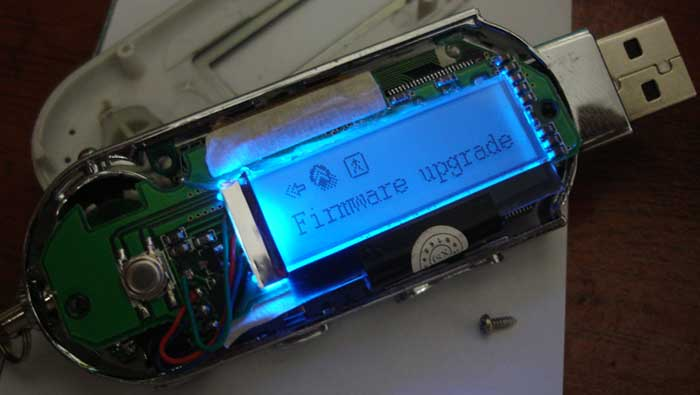
\includegraphics[height=2cm]{res/Firmware_upgrade.jpg} \cite{firmwareUpgrade}
\end{frame}

\begin{frame}{PID 1}
	Nachdem Linux alles initializiert hat wird Kontrolle an Userspace uebergeben.
	Ueblicherweise ist dies systemd.
	\begin{itemize}
		\item systemd
		\begin{itemize}
			\item einfach da bekannt
			\item wenn mehrere Dienste noetig
			\item gewisse groesse
		\end{itemize}
		\item script
		\begin{itemize}
			\item wenn nur wenige Dienste
		\end{itemize}
		\item applikation
		\begin{itemize}
			\item Applikation muss alles machen
			\item nur fuer monolithische Applikationen
		\end{itemize}
	\end{itemize}
\end{frame}

\begin{frame}{Yocto}
	Aufgaben um Embedded system zu erstellen
	\begin{itemize}
		\item Cross Compiler bauen
		\item sysfs bauen (Kernel und benoetigte Tools fuer system)
		\item Cross Compiler und sysfs fuer Developer bereitstellen (sdk)
	\end{itemize}
	Aufgaben um Embedded system zu deployen
	\begin{itemize}
		\item Applikation cross-compilen
		\item sysfs cross-compilen
		\item Kernel cross-compilen
		\item applikationen packetieren
		\item image zusammenstellen
	\end{itemize}
	daher Yocto (Yocto Workflow zeigen, resp. bild aus fsfe präsentation)
\end{frame}

\begin{frame}{Kernel / Linux}
	\begin{itemize}
		\item Verteilen von Resourcen
		\item Initialisieren und Abstrahieren der Hardware
	\end{itemize}
\end{frame}

\begin{frame}{Device Tree}
	\begin{itemize}
		\item meiste Hardware ist nicht Plug and Play
		\item wir muessen Linux mitteilen, wo welche Hardware liegt
		\item Device Tree listet auf, wo sich welche Hardware befindet
		\item Linux laedt Treiber anhand Infos in Device Tree
	\end{itemize}
	\begin{itemize}
		\item Struktur aehnlich wie XML
		\item gegliedert nach BUS
		\item beschreibt welche Hardwrae angeschlossen ist
		\item Hierarchisch aufgebaut wie Hardware (SOC, Modul, Geraet, System)
	\end{itemize}
	Beispiel
\end{frame}
